%!TEX root = ../../../../memoria.tex
\subsection{\shippingEF}\label{cap:solucionImplementada:section:dashboard:subsection:shipping}

\shippingEF es parte del proceso realmente grande y complejo perteneciente al \workflowCPT \orderFulfillmentCOM. 

Como primer paso, hay que agregar una dirección de origen, la cual es agregada en \nameref{capitulo:solucionImplementada:dashboard:subsubsection:addressPanel}.

Segundo, se deben agregar \shippingZonesCOM, los cuales tendrán su correspondiente \shippingRatesCOM. Existen servicios que permiten calcular en tiempo real el \shippingRatesCOM, evitando así que la tienda asuma un costo extra por un error en la estimación de la tarifa de envío. El sitio además debería ser capaz de determinar si la dirección de destino se encuentra dentro de alguna de las \shippingZonesCOM definidas.

% TODO falta agregar descripcion del proceso
%https://docs.shopify.com/manual/shipping/initial-shipping-setup#add-a-shipping-zone

Por temas de tiempo, se decidió simplificar la solución, permitiendo agregar diferentes opciones de \shippingEF que eventualmente representarían diferentes criterios de envío.

%TODO Agregar mas informaciñon 

\begin{figure}[H]
	\centering
	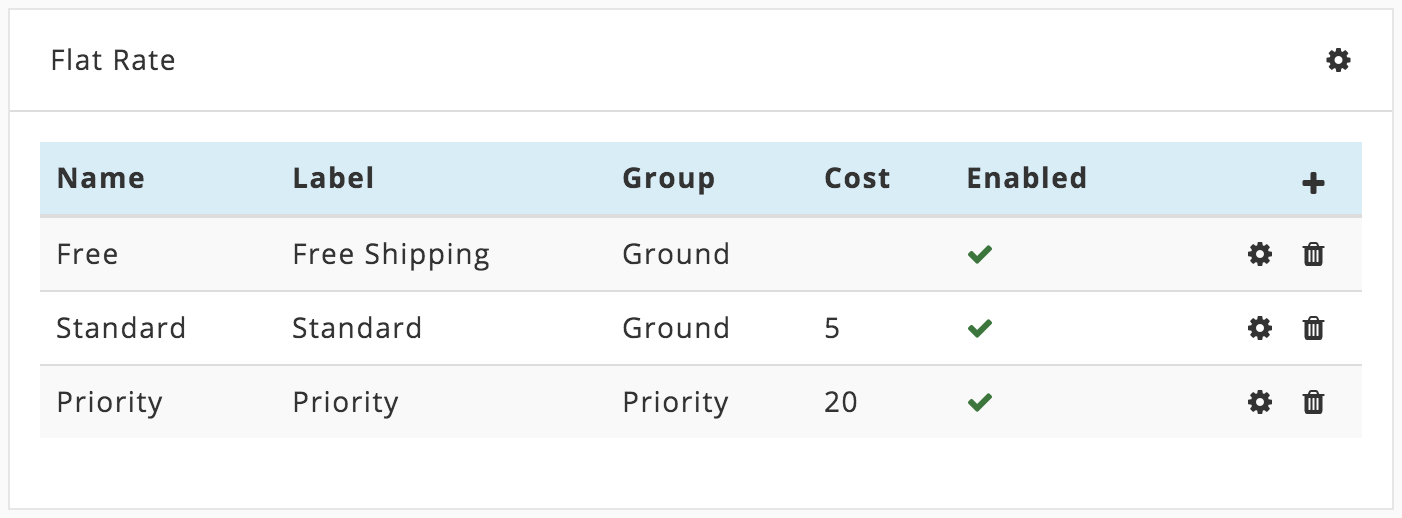
\includegraphics[width=0.6\textwidth]{figuras/dashboard/shipping/shipping_options.png}
	\caption{Tabla con todas las opciones de \shippingEF disponibles.}
	\label{figure:dashboard:shipping:shipping_options}
\end{figure}

\begin{table}[H]
    \centering
	\begin{tabular}{ |l|c||l| }
		\hline Campo & Requerido & Restricción \\ \hline
		\multirow{1}{*}{\textit{Method Name}} 	&  \checkmark 	& \\ \hline
		\multirow{1}{*}{\textit{Public Label}} 	&  \checkmark	& \\ \hline
		\multirow{1}{*}{\textit{Group}} 		&  \checkmark	& \\ \hline
		\multirow{1}{*}{\textit{Cost}} 			&  				& \\ \hline
		\multirow{1}{*}{\textit{Handling}} 		&  				& \\ \hline
		\multirow{1}{*}{\textit{Rate}} 			&  \checkmark	& Número mayor que 0. \\ \hline
		\multirow{1}{*}{\textit{Enabled}} 		&  \checkmark	& Boolean. \\ \hline
		\hline
	\end{tabular}
 	\caption{Resumen restricciones formulario para \shippingEF.}
    \label{tab:dashboard:shipping:form:restrictions:shipping}
\end{table}

\begin{figure}[H]
	\centering
	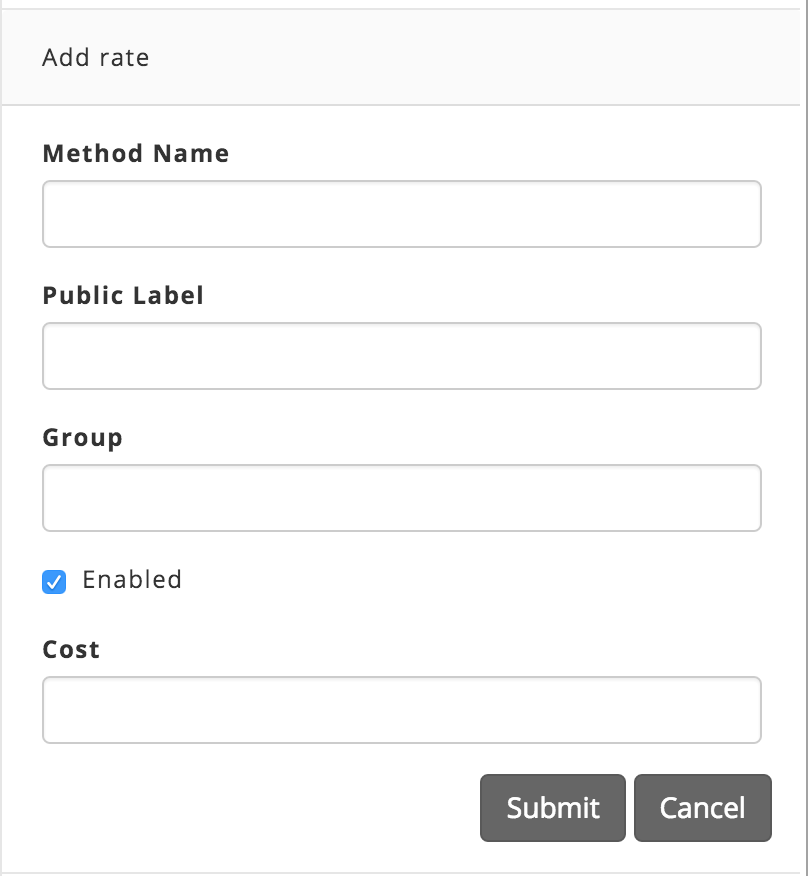
\includegraphics[width=0.6\textwidth]{figuras/dashboard/shipping/form_shipping_add.png}
	\caption{Formulario para la creación de \shippingEF.}
	\label{figure:dashboard:shipping:form_shipping_add}
\end{figure}



\begin{figure}[H]
	\centering
	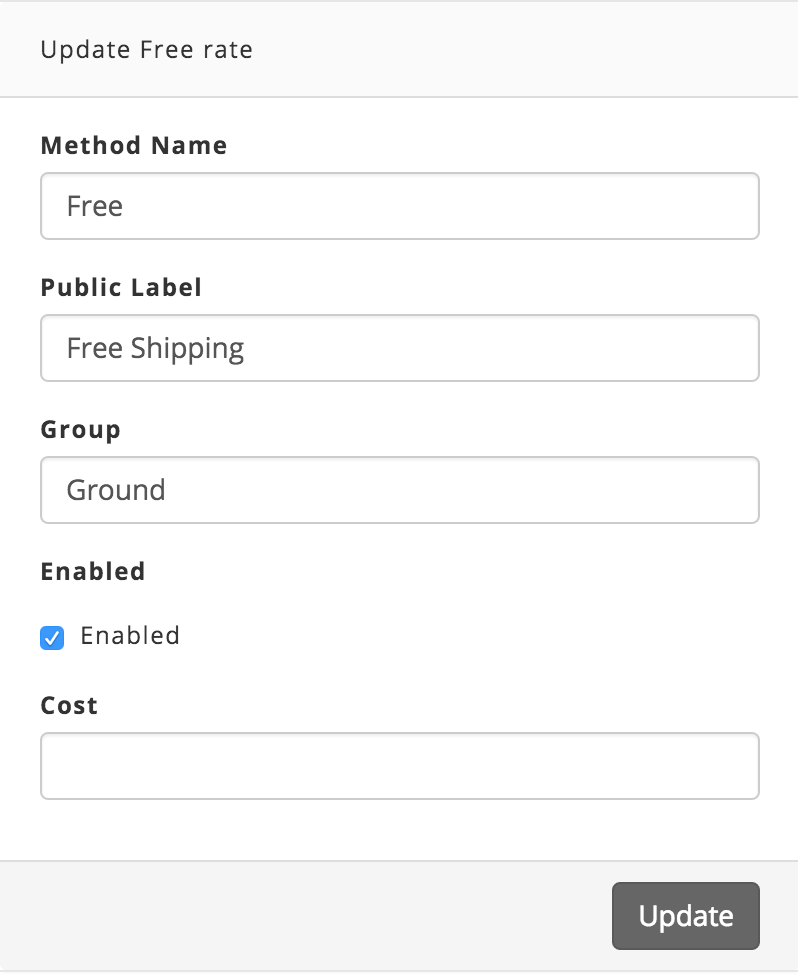
\includegraphics[width=0.6\textwidth]{figuras/dashboard/shipping/form_shipping_update.png}
	\caption{Formulario de actualización un \shippingEF.}
	\label{figure:dashboard:shipping:form_shipping_update}
\end{figure}


\subsubsection{Tarifas de \shippingEF y carros abandonados}

Aunque no es un tema que involucre a la finalidad de esta memoria, es importante mencionar la importancia que tiene el factor \shippingEF dentro del abandono del carro de compra.El desafío real que aparece cuando se desea abordar la estrategía de \shippingEF, es determinar la solución que impacte lo mínimo posible los márgenes, pero que aún así siga siendo atractivo para el cliente. Y esto es algo en lo que se desea estar en lo correcto. Estudios demuestran que el costo de \shippingEF es la principal razón del abandono de carros de compra (\refFigura{figure:dashboard:shipping:key_factor_shopping_cart_abandonment})\cite{online_forrester_consulting_smarter_stratefie_free_shipping}.

\begin{figure}[H]
	\centering
	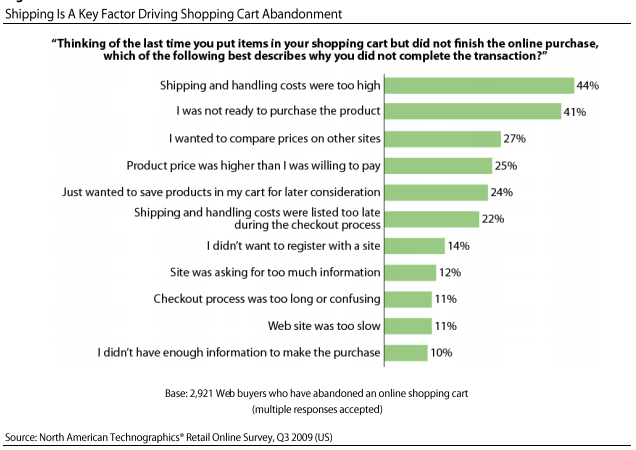
\includegraphics[width=1\textwidth]{figuras/dashboard/shipping/key_factor_shopping_cart_abandonment.png}
	\caption{\shippingEF es un factor clave en el abandono de carros de compra \cite{online_forrester_consulting_smarter_stratefie_free_shipping}.}
	\label{figure:dashboard:shipping:key_factor_shopping_cart_abandonment}
\end{figure}